\documentclass[12pt,a4paper,oneside]{article}
\usepackage[QX]{polski}

\usepackage[utf8]{inputenc}
\usepackage{latexsym}
\usepackage{tgpagella}
\usepackage{lmodern}
\usepackage{amsmath,amsthm,amsfonts,amssymb,alltt}
\usepackage{epsfig}
\usepackage{pdflscape}
\usepackage{caption}
\usepackage{indentfirst}
\usepackage{float}
%\usepackage{showkeys}
\bibliographystyle{plabbrv}


\usepackage{color}
\usepackage[polish]{babel}
\usepackage{datetime2}
\usepackage[x11names,dvipsnames,table]{xcolor}
\usepackage{hyperref}
\hypersetup{
pdfauthor={Roman Czapla, Olaf Bar},
colorlinks=True,
linkcolor=darkgray,  % color of internal links (change box color with linkbordercolor)
citecolor=BrickRed,  % color of links to bibliography
filecolor=Magenta,   % color of file links
urlcolor=BlueViolet}	%%pdfpagemode=FullScreen}

% diagramy, grafy itp.
\usepackage{tikz}
\usetikzlibrary{positioning}
\usetikzlibrary{arrows}
\usetikzlibrary{arrows.meta}
\usetikzlibrary{chains,fit,shapes,calc}
\tikzset{main node/.style={circle,fill=blue!20,draw,minimum size=1cm,inner sep=0pt}}

% algorytmy
\usepackage[linesnumbered,lined,commentsnumbered]{algorithm2e}
\SetKwFor{ForEach}{for each}{do}{end for}%
\SetKwFor{ForAll}{for all}{do}{end for}%
\newenvironment{myalgorithm}
{\rule{\textwidth}{0.5mm}\\\SetAlCapSty{}\SetAlgoNoEnd\SetAlgoNoLine\begin{algorithm}}{\end{algorithm}\rule{\textwidth}{0.5mm}}


%---------------------
\overfullrule=2mm
\pagestyle{plain}
\textwidth=15cm \textheight=685pt \topmargin=-25pt \linespread{1.3} 
\setlength{\parskip}{0pt}
\setlength\arraycolsep{2pt}
\oddsidemargin =0.9cm
\evensidemargin =-0.1cm

\captionsetup{width=.95\linewidth, justification=centering}
%---------------------




\newtheorem{tw}{Twierdzenie}[section]
\newtheorem{lem}[tw]{Lemat}
\newtheorem{co}[tw]{Wniosek}
\newtheorem{prop}[tw]{Stwierdzenie}
\theoremstyle{definition}
\newtheorem{ex}{Przykład}
\newtheorem{re}[tw]{Uwaga}
\newtheorem{de}{Definicja}[section]



\newcommand{\bC}{{\mathbb C}}
\newcommand{\bR}{{\mathbb R}}
\newcommand{\bZ}{{\mathbb Z}}
\newcommand{\bQ}{{\mathbb Q}}
\newcommand{\bN}{{\mathbb N}}
\newcommand{\captionT}[1]{\caption{\textsc{\footnotesize{#1}}}}
\renewcommand\figurename{Rys.}

\numberwithin{equation}{section}
\renewcommand{\thefootnote}{\arabic{footnote})}
%\renewcommand{\thefootnote}{\alph{footnote})}



\begin{document}

% --------------------------------------------
% Strona tytułowa
% --------------------------------------------

\thispagestyle{empty}
\begin{titlepage}
\begin{center}\Large
Uniwersytet Komisji Edukacji Narodowej w Krakowie\\
\large
Instytut Bezpieczeństwa i Informatyki\\
\vskip 10pt
\end{center}
\begin{center}
\centering 
\includegraphics[width=1.0\columnwidth]{images/logo.png}
\end{center}

\begin{center}
 {\bf \fontsize{14pt}{14pt}\selectfont PROJEKT INŻYNIERSKI \\ RAPORT Z REALIZACJI PROJEKTU\\
 }
 {\fontsize{12pt}{12pt} raport z okres: dd.mm.rrrr - dd.mm.rrrr}
\end{center}
\vskip 5pt
\begin{center}
 {\bf \fontsize{22pt}{22pt}\selectfont System rekomendacji produktów. Tworzenie algorytmu rekomendacyjnego na
 podstawie preferencji użytkowników – aplikacja przeglądarkowa}
\end{center}

\begin{center}
 {\fontsize{12pt}{12pt}\selectfont wykonany przez: }
\end{center}
\begin{center}
 {\bf\fontsize{16pt}{16pt}\selectfont Krzysztof Bielkiewicz}\\
 {\fontsize{12pt}{12pt}\selectfont Nr albumu: 156791 \\\&\\}
 {\bf\fontsize{16pt}{16pt}\selectfont Anna Nowak}\\
 {\fontsize{12pt}{12pt}\selectfont Nr albumu: XXXXX\\\&\\}
 {\bf\fontsize{16pt}{16pt}\selectfont Karol Woźniak}\\
 {\fontsize{12pt}{12pt}\selectfont Nr albumu: XXXXX}
\end{center}
\begin{center}
 {\fontsize{12pt}{12pt}\selectfont pod opieką:}\\
 {\bf\fontsize{12pt}{12pt}\selectfont dr hab. inż. Mateusz Muchacki, prof. UKEN}
\end{center}

%\mbox{}
\vspace*{\fill}
%\vskip 50pt
\begin{center}
\large
Kraków \the\year\\
(ostatnia aktualizacja: \DTMcurrenttime,\;\today)
\end{center}
\end{titlepage}
\setcounter{page}{0} 
\newpage\null\thispagestyle{empty}
%\setcounter{page}{0} 
%\newpage
%\thispagestyle{empty}

\tableofcontents


\newpage

\section{Informacja na temat postępów prac nad projektem}

\subsection{Zespół projektowy}
\textit{Lista osób tworzących zespół projektowy wraz z danymi kontaktowi (e-mail).}
    \paragraph{Grzegorz Golonka}
    \begin{itemize}
        \item E-mail:
    \end{itemize}
    \paragraph{Krzysztof Bielkiewicz}
    \begin{itemize}
        \item E-mail:  krzysztof.bielkiewicz@student.up.krakow.pl
    \end{itemize}
    \paragraph{Maciej Faber}
    \begin{itemize}
        \item E-mail:
    \end{itemize}

\subsection{Zrealizowane zadania}
\textit{Lista zrealizowanych prac z podziałem na członków zespołu projektowego.}
\paragraph{Krzysztof Bielkiewicz}
\begin{itemize}
\item Zadanie 1. Stworzenie nagłówka dla aplikacji (\hyperref[1.3.1]{sekcja 1.3.1})
\item Zadanie 2. Stworzenie strony startowej (\hyperref[1.3.2]{sekcja 1.3.2})
\item Zadanie 3. Opcja wyszukiwania po słowach kluczowych (\hyperref[1.3.3]{sekcja 1.3.3})
\item Zadanie 4. Opcja wyszukiwania po kategoriach (\hyperref[1.3.4]{sekcja 1.3.4})
\item zadanie nr 5 (\hyperref[1.3.5]{sekcja 1.3.5})
\end{itemize}
\paragraph{Anna Nowak}
\begin{itemize}
\item zadanie nr 1 (sekcja 1.3.n+1)
\item zadanie nr 2 (sekcja 1.3.n+2)
\item \dots
\item zadanie nr m (sekcja 1.3.n+m)
\end{itemize}
\paragraph{Karol Woźniak}
\begin{itemize}
\item zadanie nr 1 (sekcja 1.3.m+1)
\item zadanie nr 2 (sekcja 1.3.m+2)
\item \dots
\item zadanie nr k (sekcja 1.3.m+k)

\end{itemize}

\subsection {Opis zrealizowanych prac}
\subsubsection{Krzysztof Bielkiewicz: zadanie 1. Stworzenie nagłówka dla aplikacji}
\label{1.3.1}
\textit{Responsywny nagłówek dla całej aplikacji, co zawiera:}
\begin{itemize}
    \item Nazwe aplikacji, funkcje wyszukiwania
    \item Przycisk z wyborem kategorii i przekierowania do produktów z wybranej kategorii
    \item Przyciski przekierowania do strony z Ulubione i Koszyka
    \item Przycisk Profile pokazujący przyciski przekierowujące do:
        \begin{itemize}
            \item Edycji profilu, Dodania adresu
            \item Wiadomości, Szczegółów zamówienia
            \item Wylogowania
        \end{itemize}
\end{itemize}

\begin{figure}[H]
    \centering
    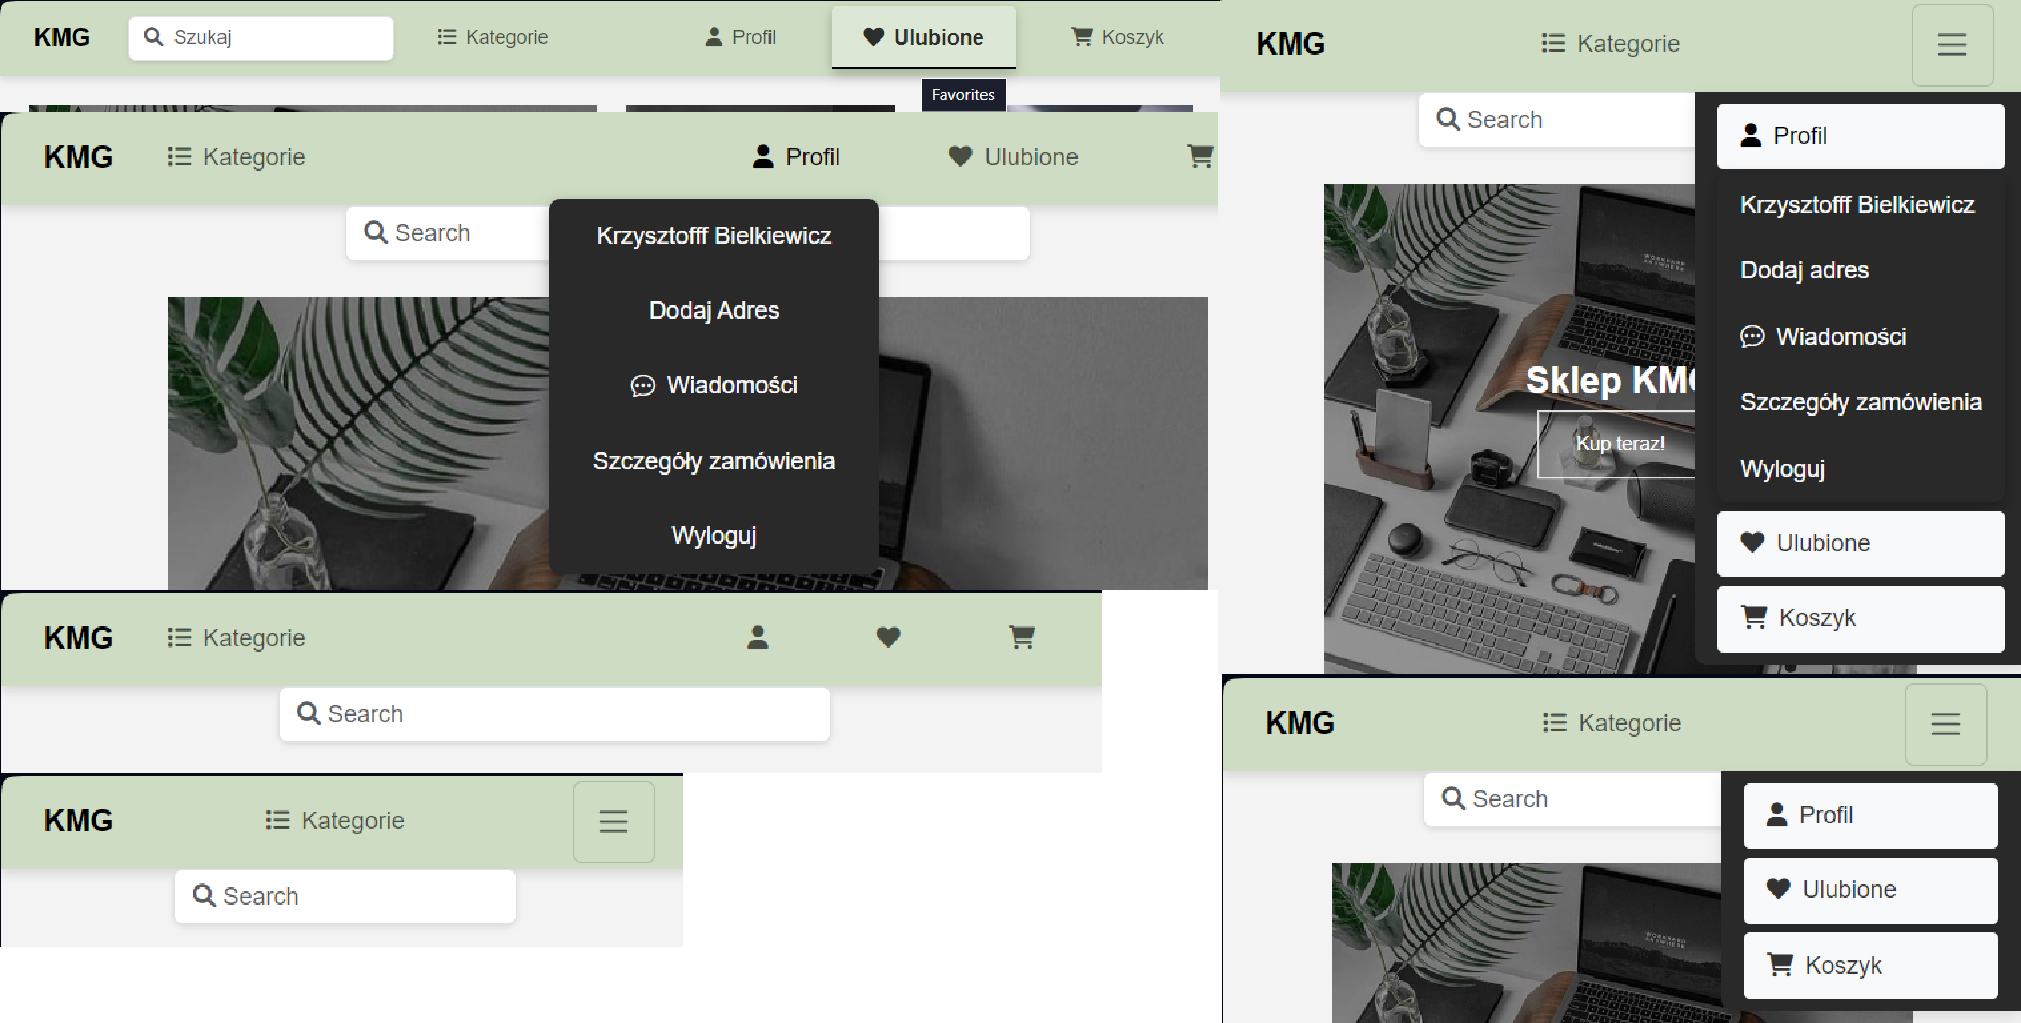
\includegraphics[width=0.9\columnwidth]{images/krzysztofBImages/header.png}
    \caption{Nagłówek z przyciskami}
    \label{header}
\end{figure}

\begin{figure}[H]
    \centering
    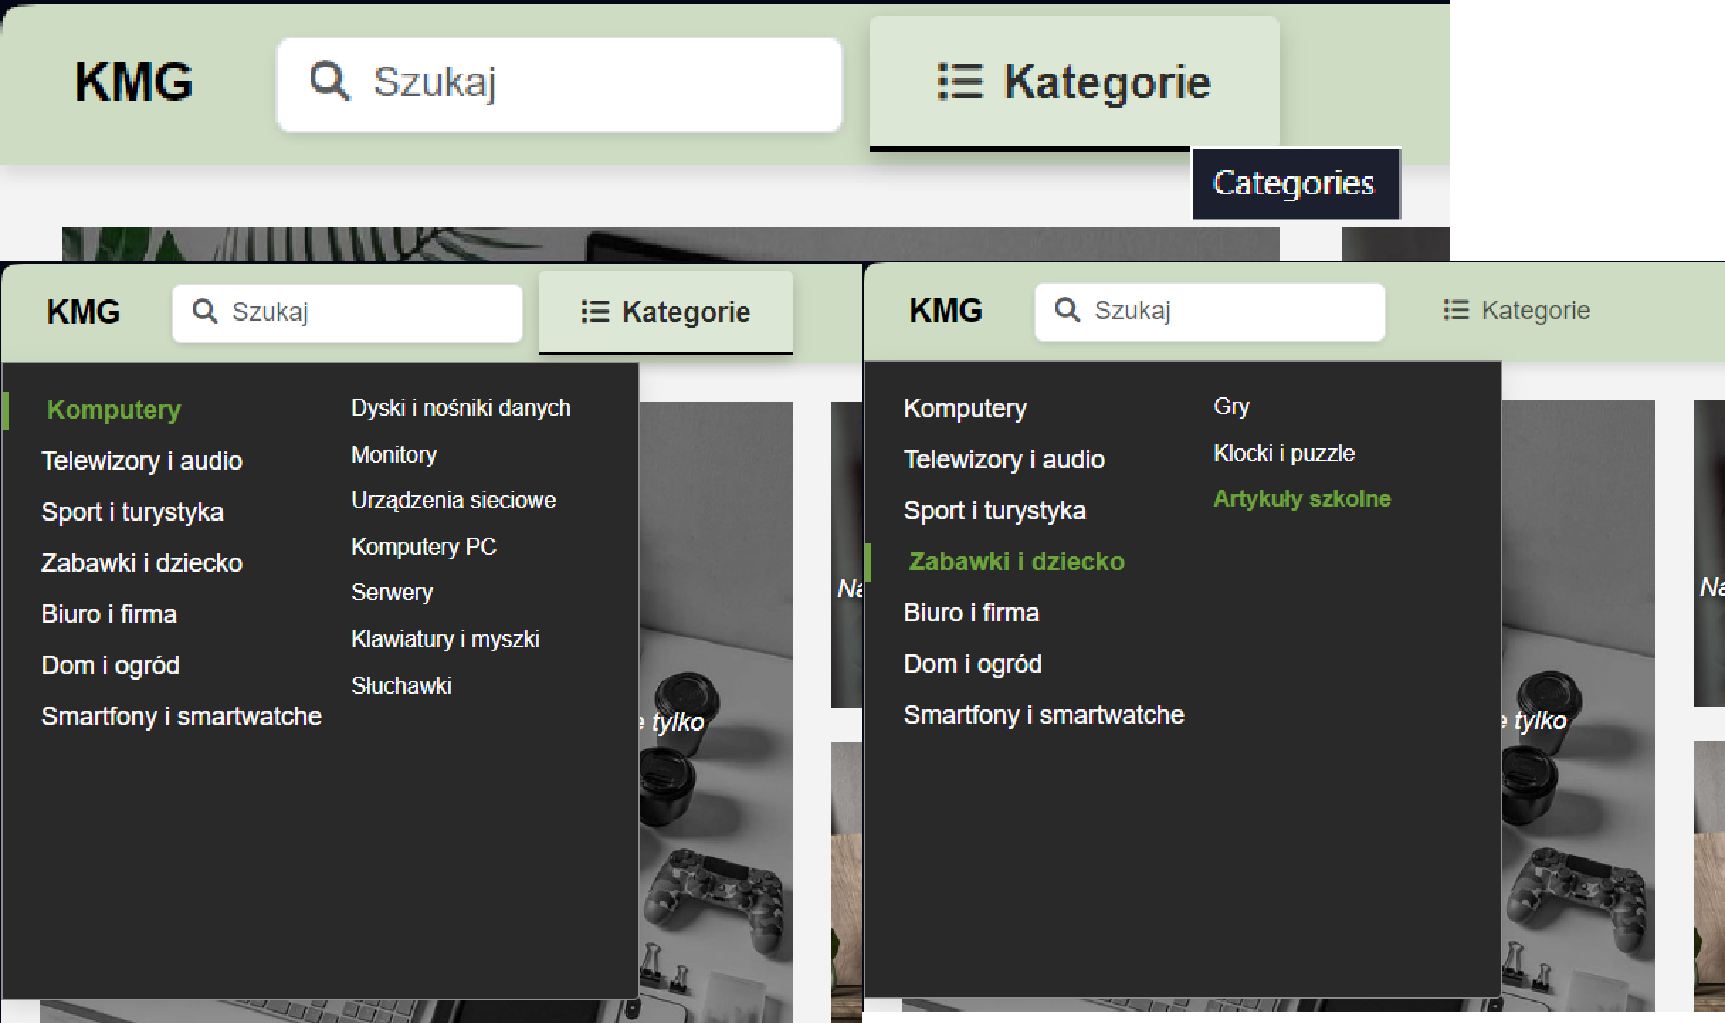
\includegraphics[width=0.9\columnwidth]{images/krzysztofBImages/header-categories.png}
    \caption{Wybór kategorii w nagłówku}
    \label{header-categories}
\end{figure}



\subsubsection{Krzysztof Bielkiewicz: zadanie 2. Stworzenie strony startowej}
\label{1.3.2}
\textit{Responsywna strona startowa zawierająca:}
    \begin{itemize}
        \item Główny baner z przekierowaniami do poszczególnych kategorii
        \item Interaktywny slider wyświetlający polecane produkty oraz drugi co wyświetla polubione produkty
        \item Stopka
    \end{itemize}
    \begin{figure}[H]
        \centering
        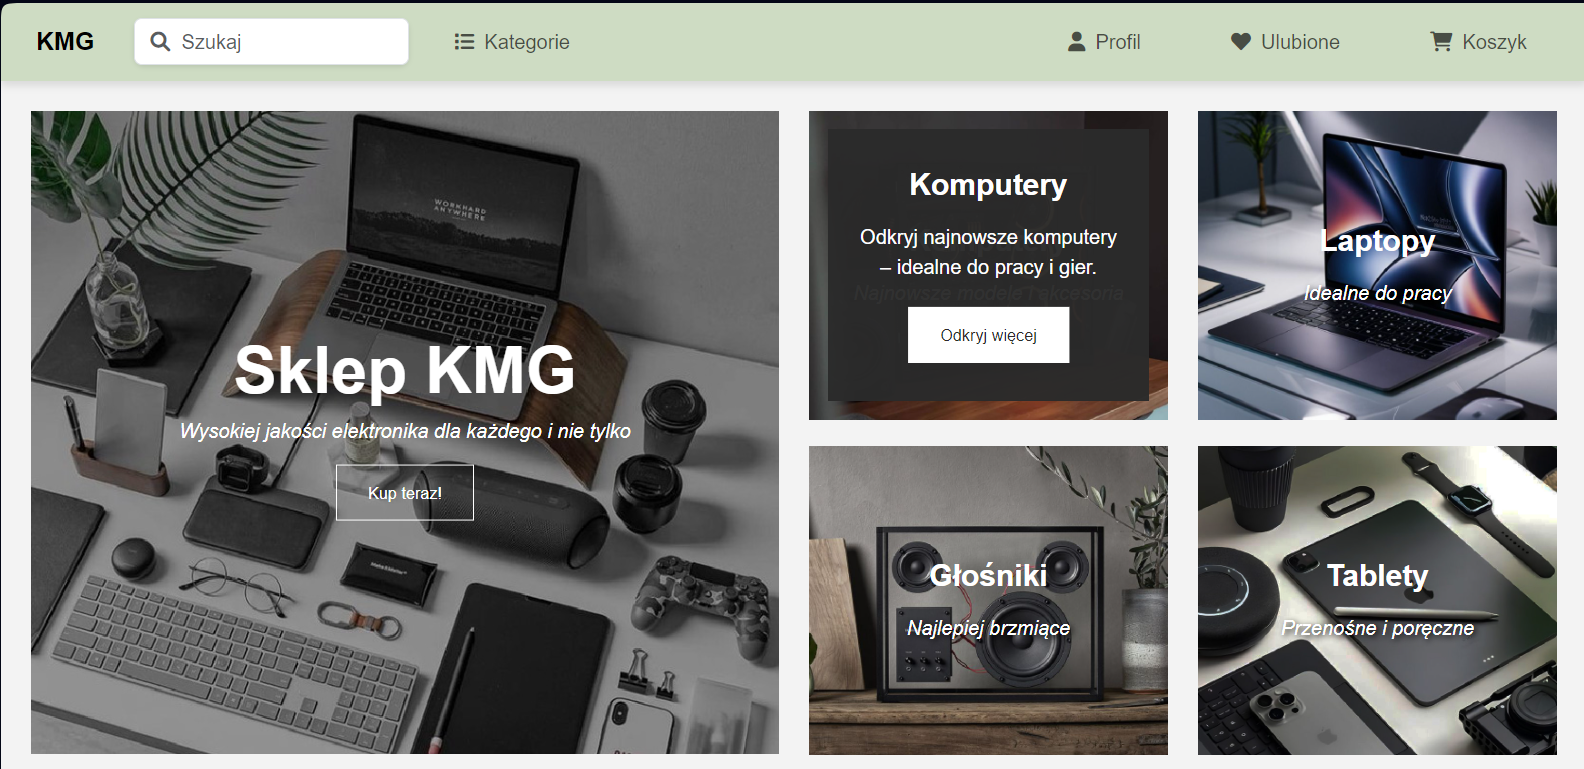
\includegraphics[width=0.8\columnwidth]{images/krzysztofBImages/main-banner.png}
        \caption{Główny banner}
        \label{main-banner}
    \end{figure}
    \begin{figure}[H]
        \centering
        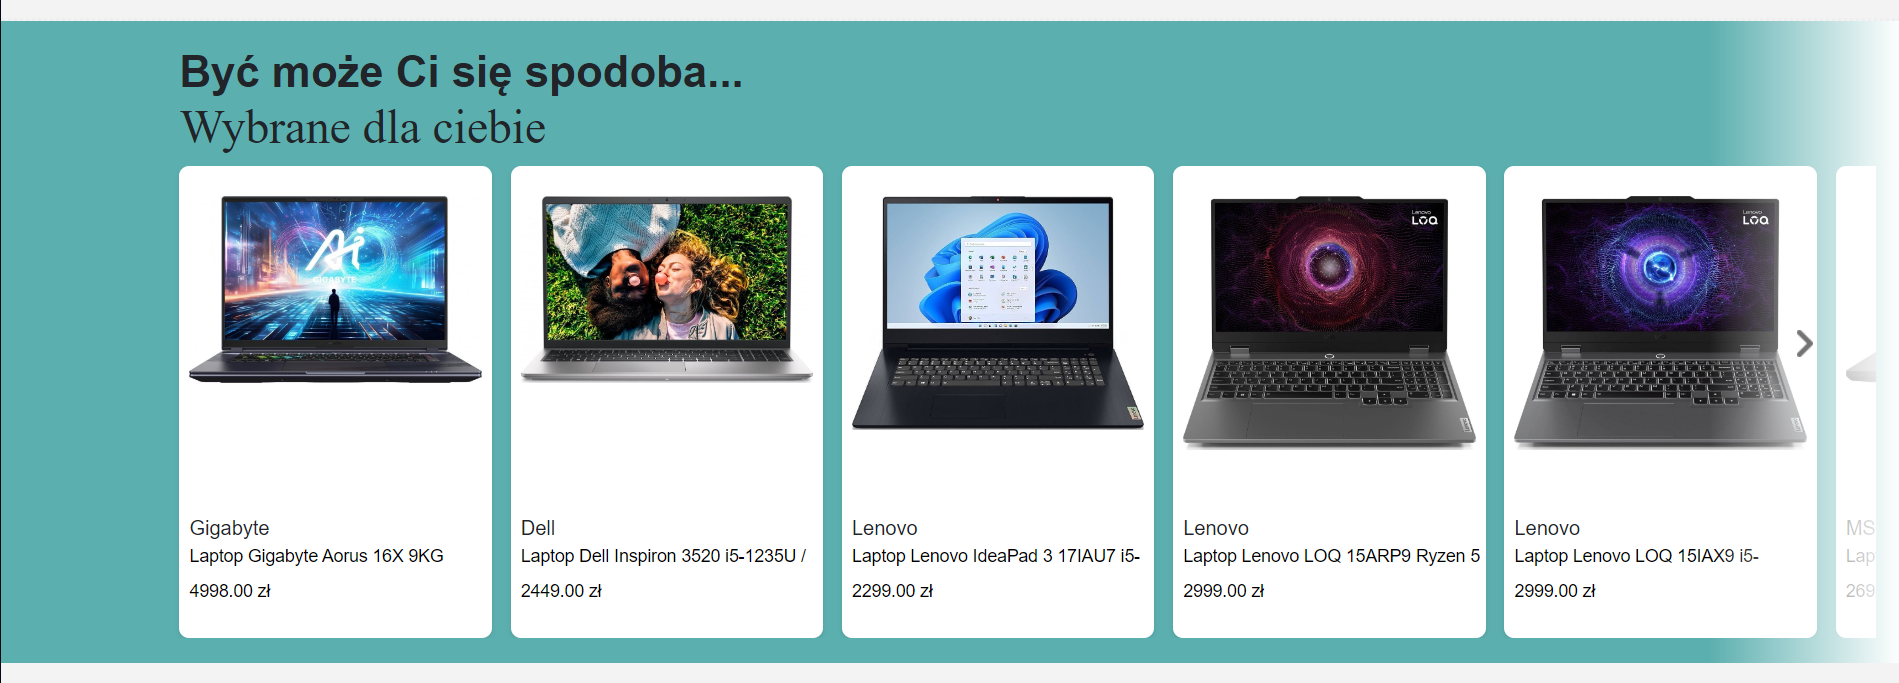
\includegraphics[width=0.8\columnwidth]{images/krzysztofBImages/slider-polecane.png}
        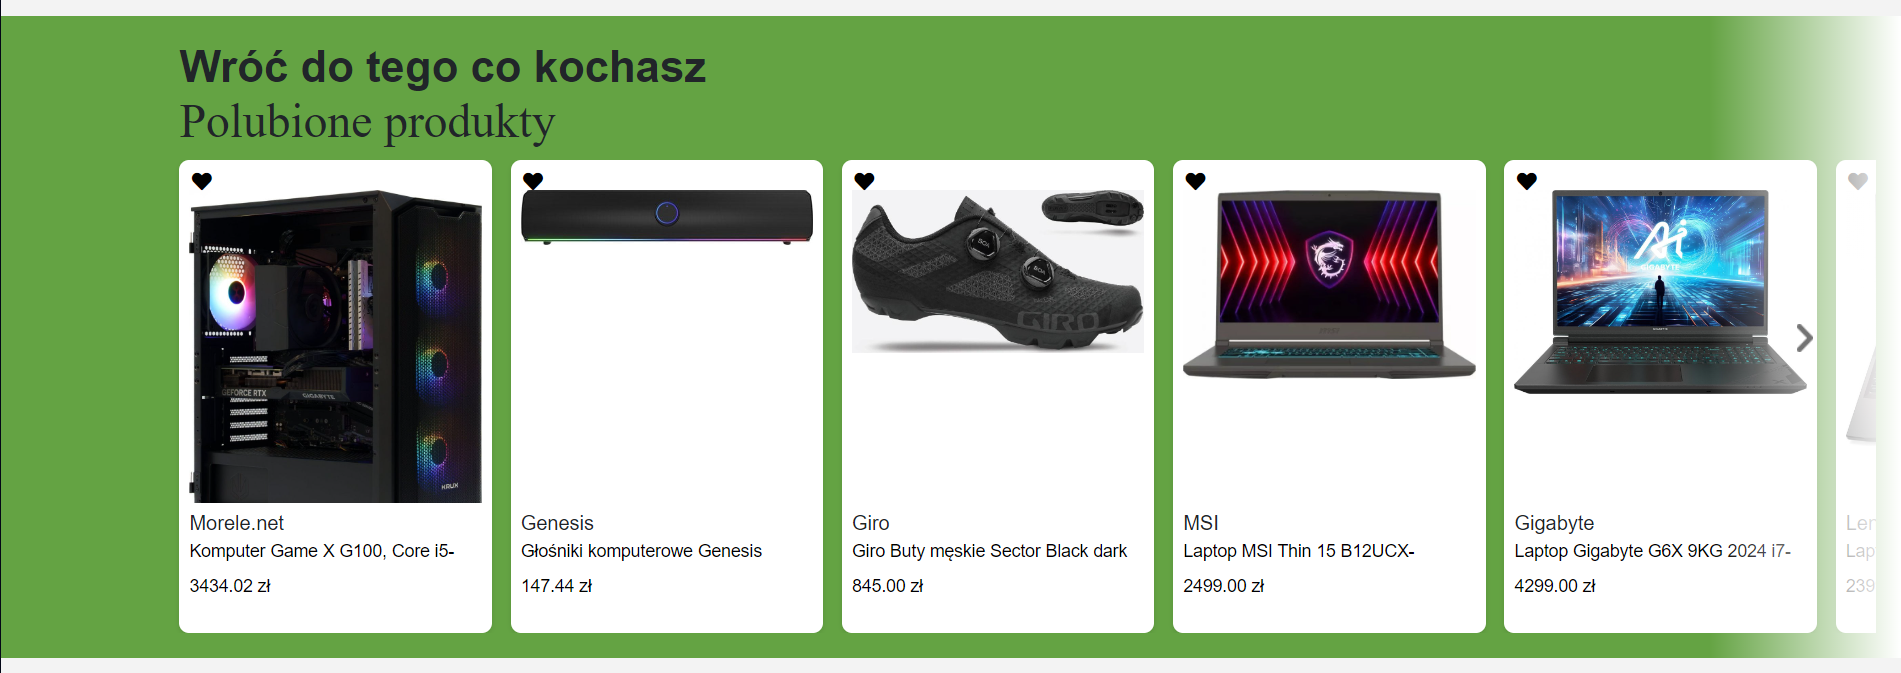
\includegraphics[width=0.8\columnwidth]{images/krzysztofBImages/slider-ulubione.png}
        \caption{Slider z polecanymi i polubionymi}
        \label{Slider}
    \end{figure}
    \begin{figure}[H]
        \centering
        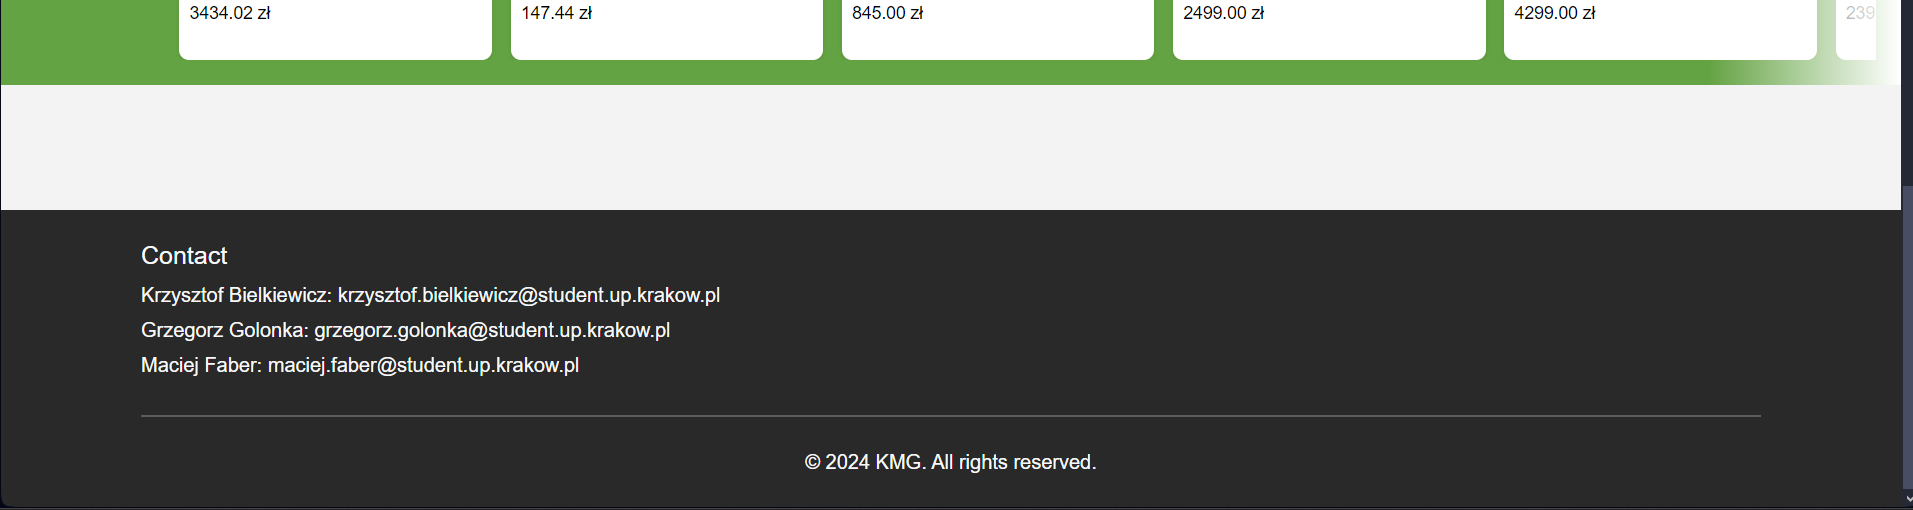
\includegraphics[width=0.8\columnwidth]{images/krzysztofBImages/footer.png}
        \caption{Stopka}
        \label{Stopka}
    \end{figure}


\subsubsection{Krzysztof Bielkiewicz: zadanie 3. Opcja wyszukiwania po słowach kluczowych}
\label{1.3.3}
\textit{Implementacja w backend wyszukiwania po słowach wpisanych w rubryce 'Szukaj'
oraz strona wyświetlająca wynik wyszukiwania}
\begin{figure}[H]
    \centering
    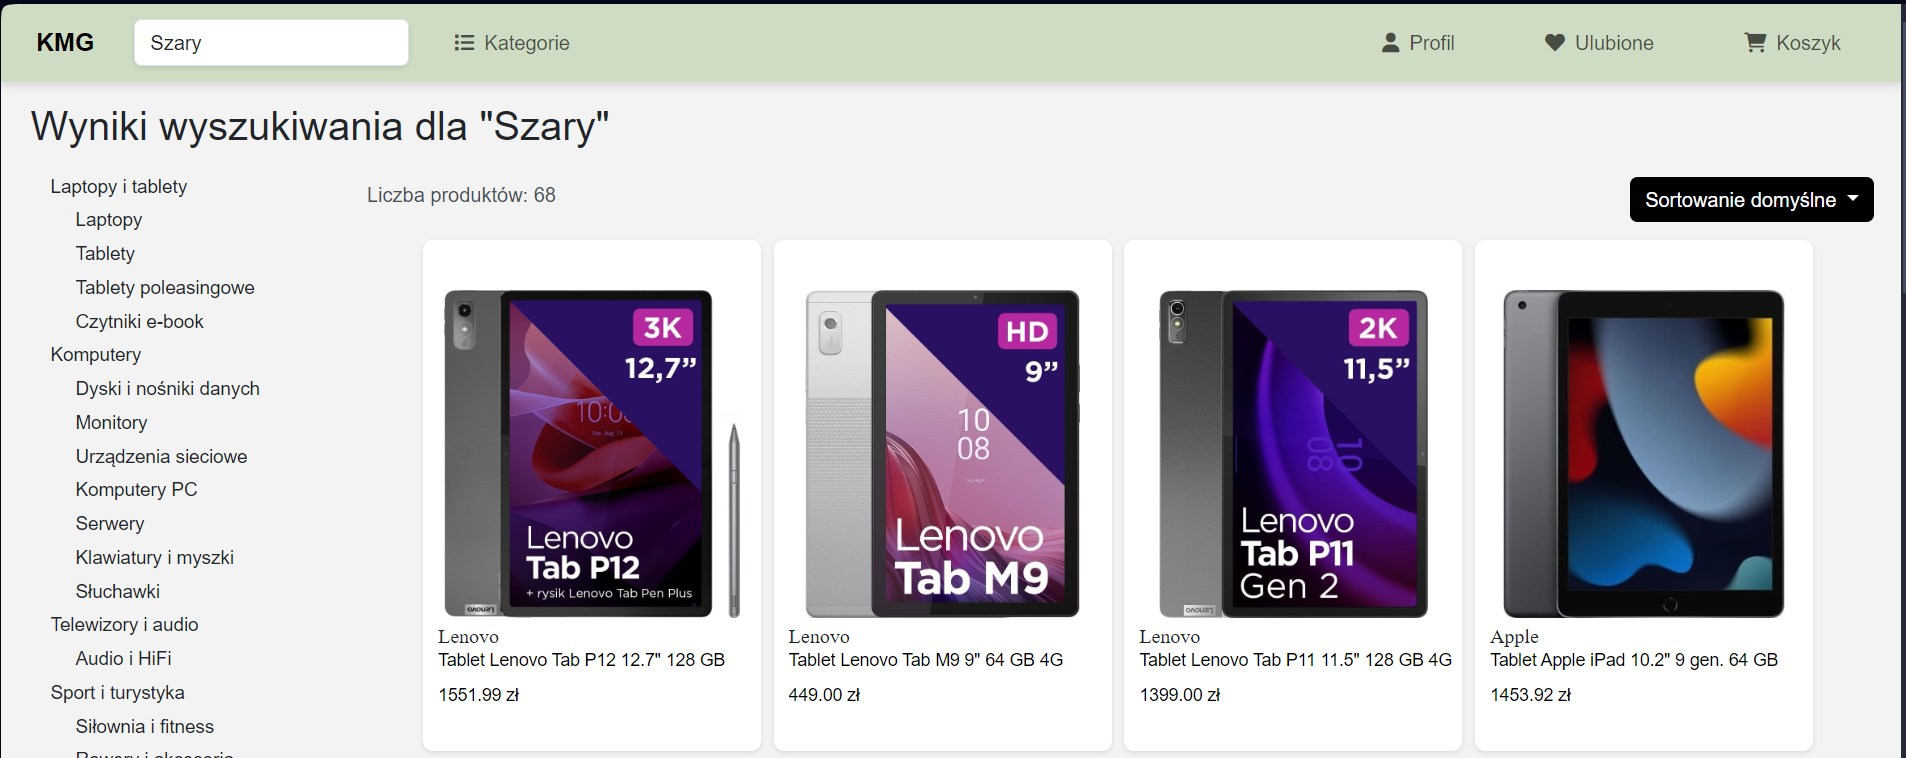
\includegraphics[width=0.8\columnwidth]{images/krzysztofBImages/wyszukiwanie.png}
    \caption{Wynik wyszukiwania}
    \label{search-value}
\end{figure}

    
\subsubsection{Krzysztof Bielkiewicz: zadanie 4. Opcja wyszukiwania po kategoriach}
\label{1.3.4}
    \textit{Zaimplementowana w backend opcja wyszukiwania po kategoriach
     oraz stworzenie w frontend liste kategorii w nagłówku
      oraz liste kategorii po lewej stronie od wyświetlanych produktów w której jest zaznaczona
      aktualnie przeglądana kategoria. Utworzenie strony z wyświetlanymi produktami z wybranej kategorii.}
    \begin{center}
        \hyperref[header-categories]{Zdjęcie wyszukiwania po kategoriach w nagłówku}
    \end{center}

    \begin{figure}[H]
        \centering
        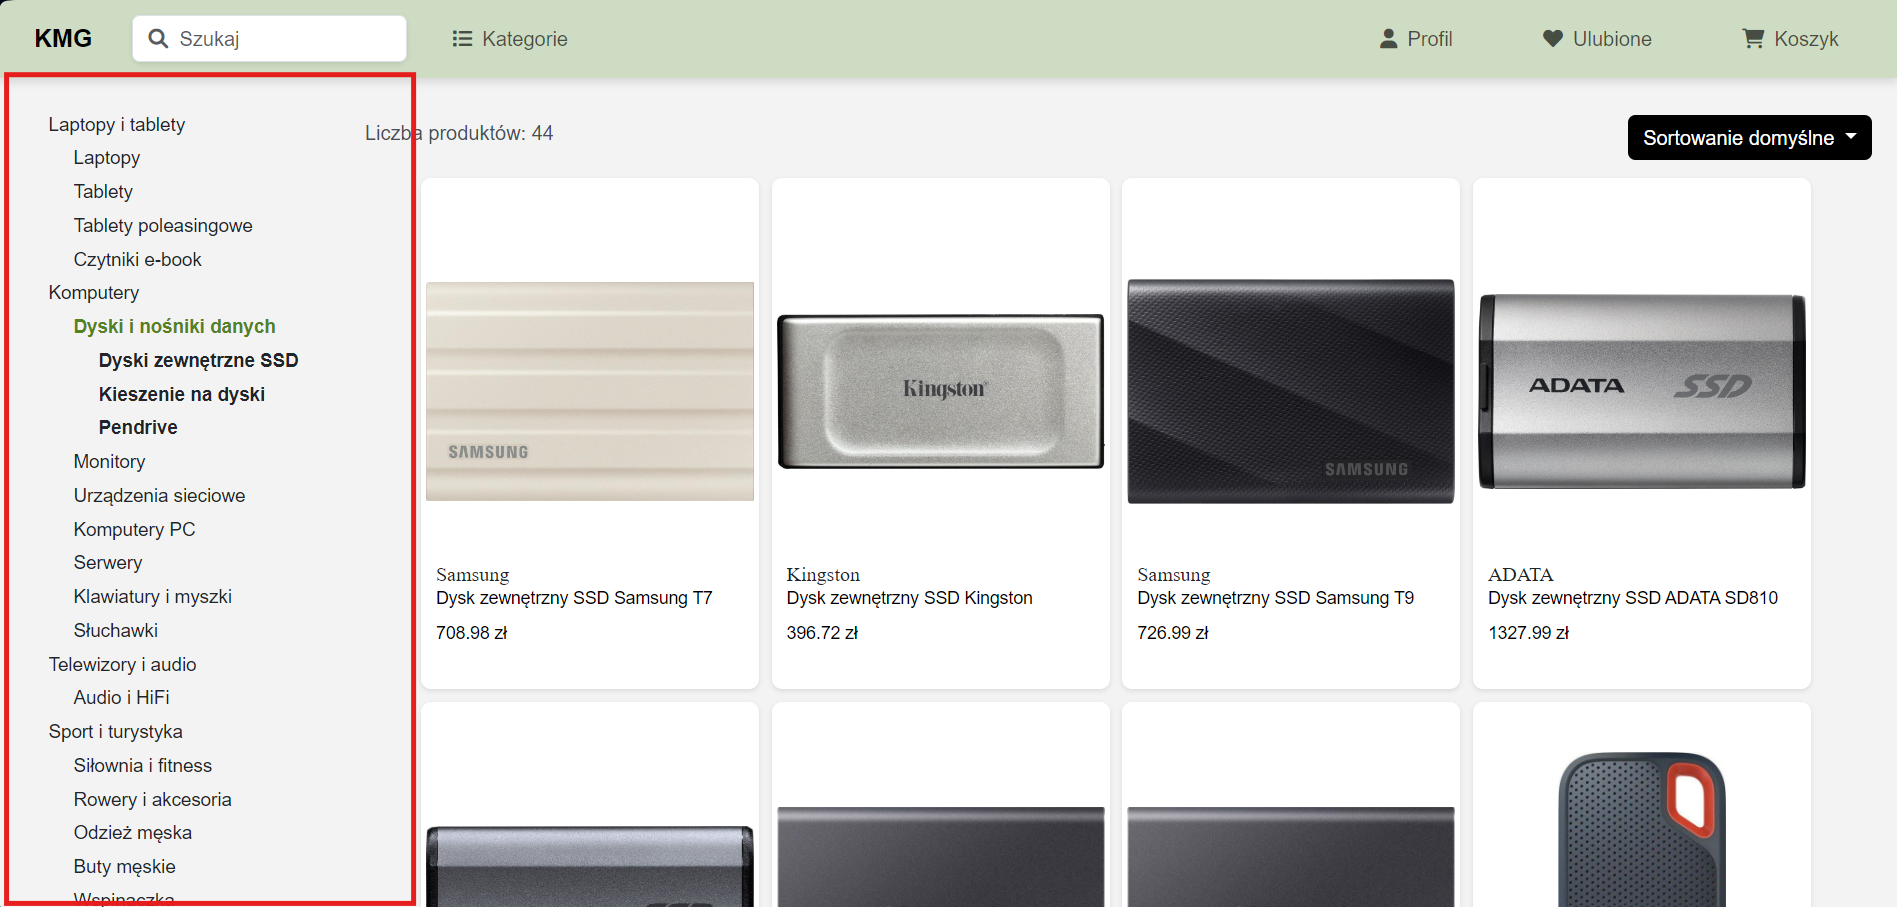
\includegraphics[width=0.8\columnwidth]{images/krzysztofBImages/lewe-kategorie.png}
        \caption{Kategorie po lewej stronie na stronie z produktami z wybranej kategorii}
        \label{left-categories}
    \end{figure}




\subsubsection{Krzysztof Bielkiewicz: zadanie nr 5}
\label{1.3.5}
\textit{Krótkie wyjaśnienie, opis lub odwołanie do załącznika.}


\subsubsection{Anna Nowak: zadanie nr 1}
\textit{Krótkie wyjaśnienie, opis lub odwołanie do załącznika.}
\subsubsection{Anna Nowak: zadanie nr 2}
\textit{Krótkie wyjaśnienie, opis lub odwołanie do załącznika.}


\subsubsection{Karol Woźniak: zadanie nr 1}
\textit{Krótkie wyjaśnienie, opis lub odwołanie do załącznika.}
\subsubsection{Karol Woźniak: zadanie nr 2}
\textit{Krótkie wyjaśnienie, opis lub odwołanie do załącznika.}

\subsection{Załączniki}
\textit{Lista załączników lub dodatkowych materiałów potwierdzających zrealizowane zadania.}



\renewcommand\refname{Literatura (jeżeli wymagana)}
\bibliography{references}
\addcontentsline{toc}{section}{Literatura}
% --------------------------------------------------------------------
%%%%%%% odkomentować gdy bibliografia ma być wewnątrz dokumentu
% --------------------------------------------------------------------
%\begin{thebibliography}{11}
%
%\addcontentsline{toc}{section}{Literatura}
%
%\bibitem{ZAN}
%C. Zannoni and P. Pasini, 
%\emph{Advances in the Computer Simulatons of Liquid Crystals}, Kluwer Academic Publishers, 2000.
%
%\end{thebibliography}

\end{document}

